\documentclass[8pt]{beamer}

\usetheme{Madrid}
\usecolortheme{crane}
\linespread{1.5}

\usepackage{graphicx}
\usepackage{physics}
\usepackage{hyperref}
\usepackage{slashed}
\usepackage{siunitx}
\usepackage{lmodern}
\usepackage{multicol}
\usepackage[compat=1.1.0]{tikz-feynman}

%\newcommand{\phanitem}{\phantom{\item}}
\newcommand{\gm}{\gamma^{\mu}}
\newcommand{\gn}{\gamma^{\nu}}
\newcommand{\gs}{\gamma^{\sigma}}
\newcommand{\gr}{\gamma^{\rho}}
\newcommand{\gnr}{g^{\nu\rho}}
\newcommand{\gmr}{g^{\mu\rho}}
\newcommand{\gms}{g^{\mu\sigma}}
\newcommand{\gns}{g^{\nu\sigma}}
\newcommand{\vbp}{\vb{p}}
\newcommand{\vbk}{\vb{k}}
\newcommand{\g}{\gamma}
\renewcommand{\a}{\alpha}
\renewcommand{\b}{\beta}
\renewcommand{\t}{\theta}
\newcommand{\la}{\lambda}
\newcommand{\p}{\phi}
\newcommand{\vp}{\varphi}
\newcommand{\s}{\sigma}
\newcommand{\G}{\Gamma}
\newcommand{\pars}{\slashed\partial}
\newcommand{\ps}{\slashed p}
\newcommand{\ks}{\slashed k}
\newcommand{\bP}{\vb{P}}
\newcommand{\bA}{\vb{A}}
\newcommand{\ba}{\boldsymbol{\alpha}}
\newcommand{\apo}{\abs{\vb{p}_1}}
\newcommand{\aps}{\abs{\vb{p}_2}}
\newcommand{\lag}{\mathcal{L}}
\title{Hadron Spectroscopy: Final Report}
\author{Yingsheng Huang}
\institute{Institute of High Energy Physics}
\begin{document}
\maketitle
\begin{frame}
  \frametitle{$D_1\rightarrow D^*\pi(1^+\rightarrow 1^-0^-)$}
  %\twocolumn
  %\begin{minipage}[t]{0.49\textwidth}
  \begin{multicols}{2}
    $$A_H=\sqrt{\frac{2J_1+1}{4\pi}}A_{\lambda_2\lambda_3}D^{s_1^*}_{m_1\la_2-\la_3}(\theta,\phi)$$
    $$A_{\la_2\la_3}\approx \abs{\mathbf{p}}^L,A_{10}=+A_{-10},A_{00}=+A_{00}$$
    $$A_{m'm}=\eta_{D_1}\eta_{D^*}\eta_{\pi}(-1)^{S_{D_1}-s_{D^*}-s_{\pi}}A_{-m'm}$$
    (where parity conservation is applied.)

    In this scenario, $J_1=1$, $m_1=1$, $\la_3=0$, we can choose $\la_2$ from -1 to 1. The orbital angular momentum of final states $L$ is then zero.

    $$A_H=\begin{cases}
    \frac{1}{2} \sqrt{\frac{3}{\pi }} e^{i \phi } \cos ^2\left(\frac{\theta }{2}\right), \la_2=1\\
    \sqrt{\frac{3}{2 \pi }} \sin \left(\frac{\theta }{2}\right) \cos \left(\frac{\theta }{2}\right),\la_2=0\\
    \frac{1}{2} \sqrt{\frac{3}{\pi }} e^{-i \phi } \sin ^2\left(\frac{\theta }{2}\right),\la_2=-1
  \end{cases}$$

    The differential cross section is then the square of $A_H$.
\begin{align*}
  &\dv{\Gamma_{110}}{\theta}=\frac{3 \left\left| \cos \left(\frac{\theta }{2}\right)\right\right| ^4}{4 \pi },\\
  &\dv{\Gamma_{100}}{\theta}=\frac{3 \left\left| \cos \left(\frac{\theta }{2}\right) \sin \left(\frac{\theta }{2}\right)\right\right| ^2}{2 \pi },\\
  &\dv{\Gamma_{1-10}}{\theta}=\frac{3 \left\left| \sin \left(\frac{\theta }{2}\right)\right\right| ^4}{4 \pi }$$
\end{align*}
    %$$\dv{\Gamma}{\theta}=\frac{3 \left(\sqrt{2} \left| \sin (\theta )\right| +2\right)^2}{16 \pi }$$

  %\end{minipage}
  %\begin{minipage}[t]{0.49\textwidth}
  %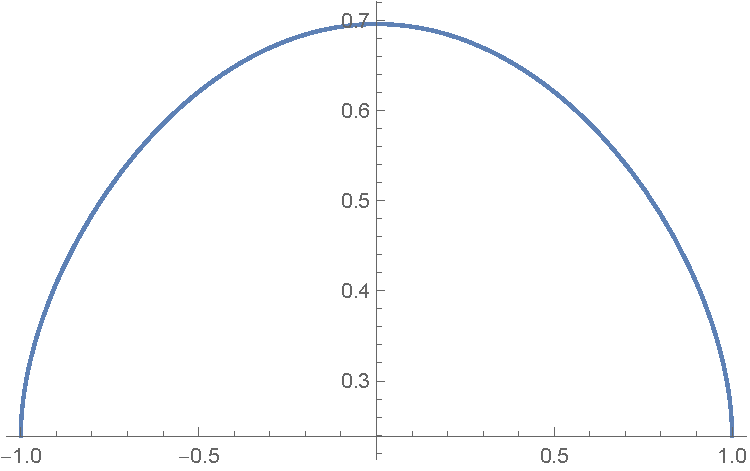
\includegraphics[width=0.45\textwidth]{AngularDis.pdf}
  %\end{minipage}
\end{multicols}
\end{frame}
\begin{frame}
  \frametitle{$D_1\rightarrow D^*\pi_2\rightarrow (D\pi_1)\pi_2$ with another decay $D^*\rightarrow D\pi(1^-\rightarrow 0^-0^-)$}
  $$A_{H1}=\sqrt{\frac{2J_1+1}{4\pi}\frac{2J_2+1}{4\pi}}\sum_{\la_2}A_{\lambda_2\lambda_3}B_{\la_4\la_5}D^{s_1^*}_{m_1\la_2-\la_3}(\theta,\phi)D^{s_2^*}_{\la_2\la_4-\la_5}(\theta',\phi')$$
  Thus obtain:
  $$\dv{\Gamma}{\theta}=\frac{9 \left\left|e^{i\phi} p \sin \left(\frac{\theta }{2}\right) \sqrt{2} \cos ^3\left(\frac{\theta }{2}\right)-\sqrt{2} p \sin ^3\left(\frac{\theta }{2}\right) \cos \left(\frac{\theta }{2}\right)+b p \cos (\theta ) \sin \left(\frac{\theta }{2}\right) \sqrt{2} \cos \left(\frac{\theta }{2}\right)\right\right| ^2}{16 \pi ^2}$$
  %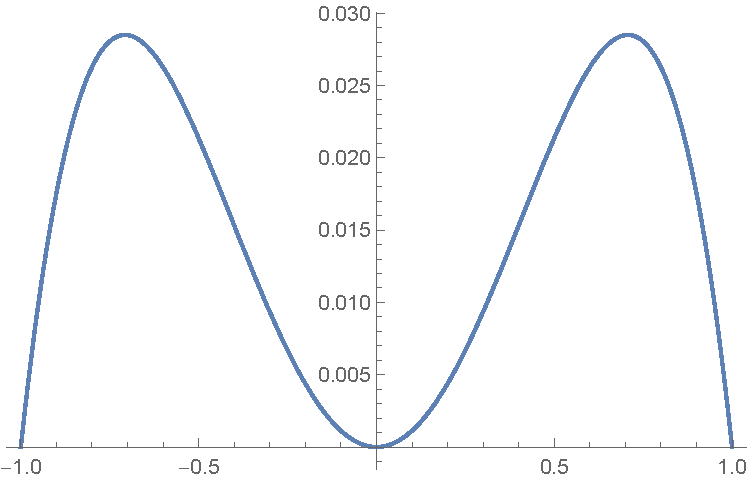
\includegraphics[width=0.28\textwidth]{AngularDis1.pdf}
  \begin{multicols}{2}
      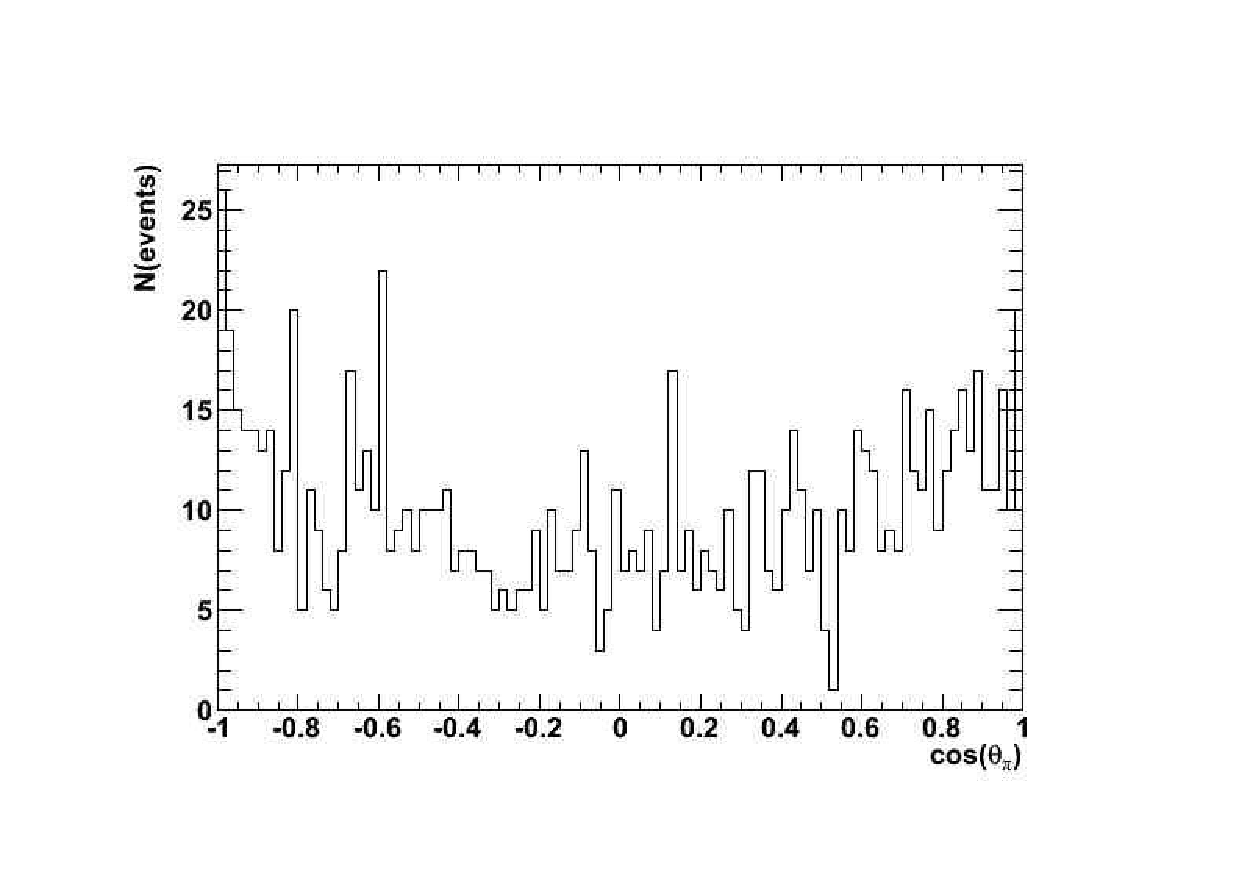
\includegraphics[width=0.5\textwidth]{HS1.pdf}

      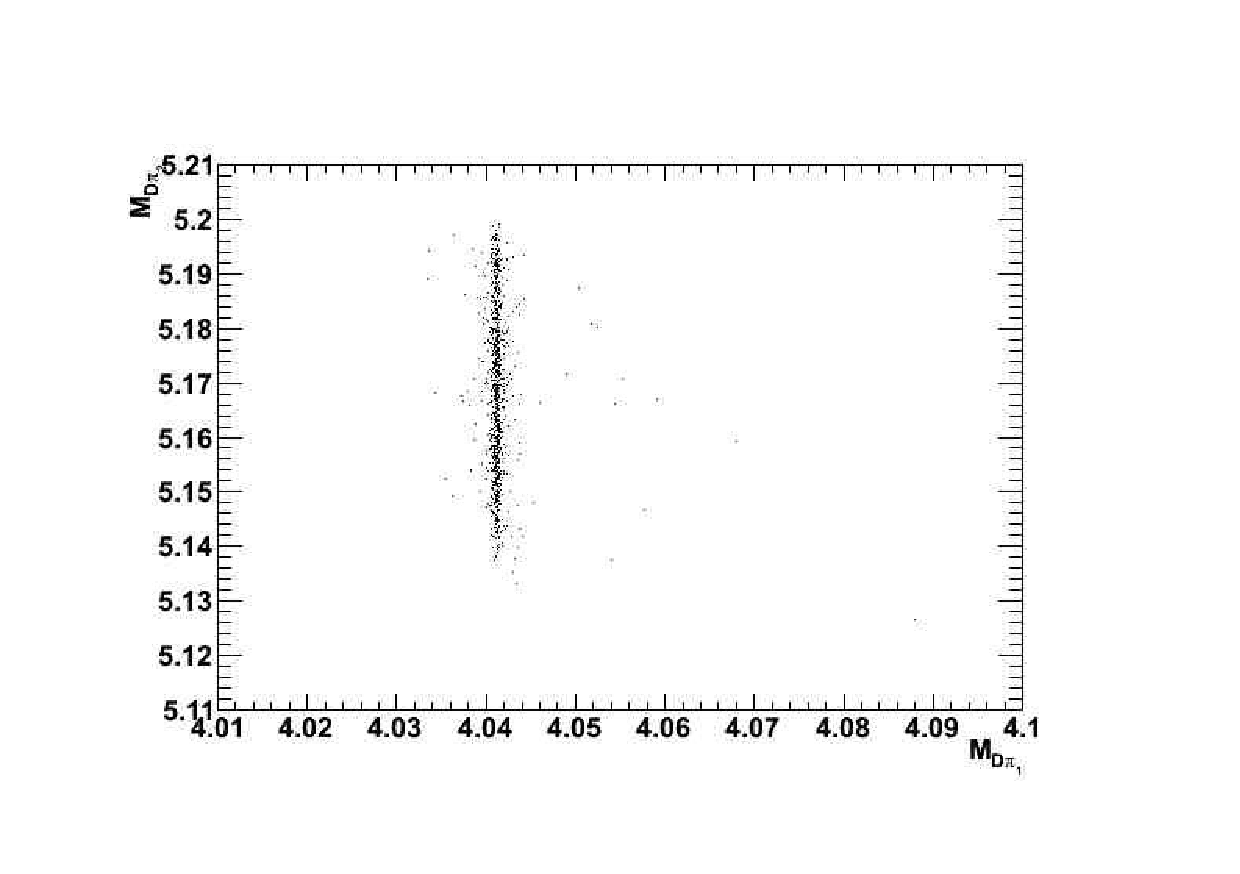
\includegraphics[width=0.5\textwidth]{HS2.pdf}
  \end{multicols}
\end{frame}
\begin{frame}
  \begin{multicols}{2}
    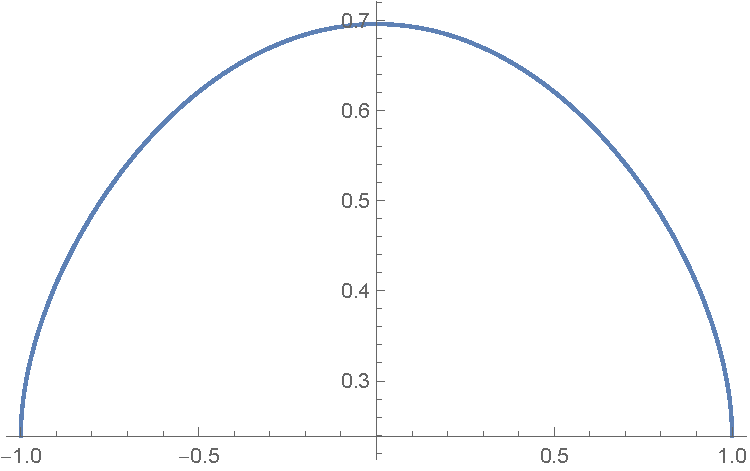
\includegraphics[width=0.45\textwidth]{AngularDis.pdf}

    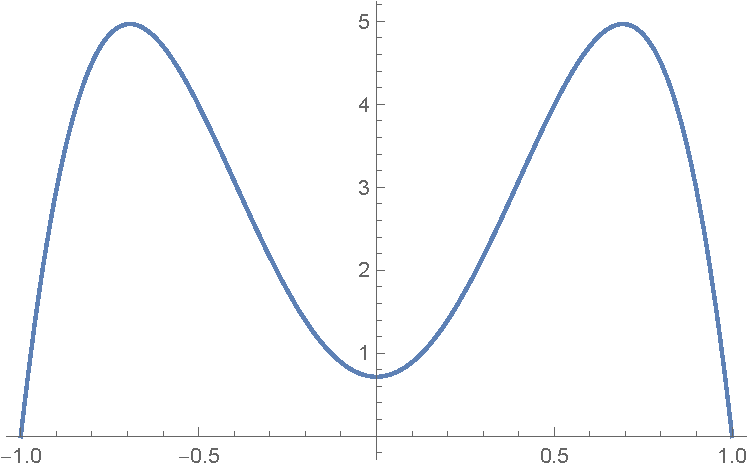
\includegraphics[width=0.45\textwidth]{AngularDis2.pdf}
  \end{multicols}
\end{frame}
\begin{frame}
  \frametitle{Landau-Yang Theorem}
  For any vector particles,we can always write the field operator as a single vector field.
  $$A_{\mu}(x)=\int\frac{\dd^3k}{(2\pi)^3}\frac{1}{\sqrt{2\abs{\vb{k}}}}\sum_{\la}(a^{\la}_{\vbk}\epsilon^{\la}_{\mu}(k)e^{-ik\cdot x}+{a^{\la}_{\vbk}}^{\dagger}{\epsilon^{\la}_{\mu}}^*(k)e^{ik\cdot x})$$
  Then the feynman rules can be easily derived. The amplitude of $vector\rightarrow \g\g$ is
  \begin{align*}
    i\mathcal{M}&=\epsilon_1^{*\mu}(p_1)\epsilon_2^{*\nu}(p_2)\epsilon^{\a}(p)\Gamma_{\mu\nu\s}\\
    \intertext{since it must obey Lorentz-invariant}
    &=(\epsilon_1\cdot\epsilon_2)(a_1\epsilon\cdot p_1+a_2\epsilon\cdot p_2)+a_3(\epsilon_1\cdot \epsilon)(\epsilon_2\cdot p_1)+a_4(\epsilon_2\cdot \epsilon)(\epsilon_1\cdot p_2)\\
    \intertext{final states symmetry (identical), $a_1=a_2$, first term vanishes. And $\epsilon_2\cdot p_1=\epsilon_1\cdot p_2=0$}
    &=0
  \end{align*}
\end{frame}
\begin{frame}
  \frametitle{R value: $e^+e^-\rightarrow hadron$}
  \begin{multicols}{2}
  Provide $s\ll m_{\mu}$,

  $$\abs{\feynmandiagram[horizontal=a to b,baseline=(a.base),small]{i1[particle=\(e^-\)]--[fermion]a--[fermion]i2[particle=\(e^+\)],f1[particle=\(\mu^-\)]--[fermion]b--[fermion]f2[particle=\(\mu^-\)],a--[photon]b};}^2
%$$\feynmandiagram[horizontal=a to b,baseline=(a.base),small]{i1--[fermion]a--[fermion]i2,f1--[fermion]b--[fermion]f2,a--[photon]b};
 =\frac{4e^4}{s}(1+\cos\theta)$$
  %For hadron final states,
%  $$\feynmandiagram[horizontal=a to b,baseline=(a.base),small]{i1[particle=\(e^-\)]--[fermion]a--[fermion]i2[particle=\(e^+\)],f1[particle=\(q^-\)]--[fermion]b[blob]--[fermion]f2[particle=\(q^-\)],a--[gluon]b};\propto-i\eta_sg_s\gm T^a_{ij}$$
  Weak processes supressed when $s\ll m_Z$.

  The contribution of EM process is obvious:
  $$\feynmandiagram[horizontal=a to b,baseline=(a.base),small]{i1[particle=\(e^-\)]--[fermion]a--[fermion]i2[particle=\(e^+\)],f1[particle=\(q^-\)]--[fermion]b[blob]--[fermion]f2[particle=\(q^-\)],a--[photon]b};\propto-i\eta_eeQ_f\gm$$
\end{multicols}
\end{frame}


\end{document}
